\chapter{Getting Started}
Embedded systems \parencite{leveson_embedded_2003} are special-purpose computer systems---composed of a processor, memory, software, and peripherals for input and ouput---that are embedded into a larger mechanical or electronic system.
Embedded systems are different from general-purpose computers such as desktops, laptops, mobile phones, and tablets because they typically run a single program which is tightly integrated to the accompanying hardware it is embedded within.
Their function is often to control or monitor a machine, which requires their program to react in real-time to sensor information or user input.

According to its \href{https://www.arduino.cc/en/Guide/Introduction}{official website}, 
``Arduino is an open-source electronics platform based on easy-to-use hardware and software'' \parencite{arduino_what_2018}.
It comprises of three main elements: 
hardware boards, the most famous of which is the Arduino Uno, shown in Fig.~\ref{fig:arduino_uno};
a microcontroller programming interface and libraries, known as the \emph{Arduino language};
and an integrated development environment, the Arduino IDE.
Its low price, usability, and extensive community support make it an excelent entry point for learning embedded systems and an rapid prototyping tool for experts.

\section{Embedded Systems}
\section{Hello World on the Wokwi Simulator}
The simplest way to get started with the Arduino, for the purpose of understanding the C++ language, is using the Wokwi online electronics simulator at \href{https://wokwi.com}{wokwi.com}.
To begin, open the Hello World program shown in 

\begin{figure}
  \begin{wide}
    \hfill
    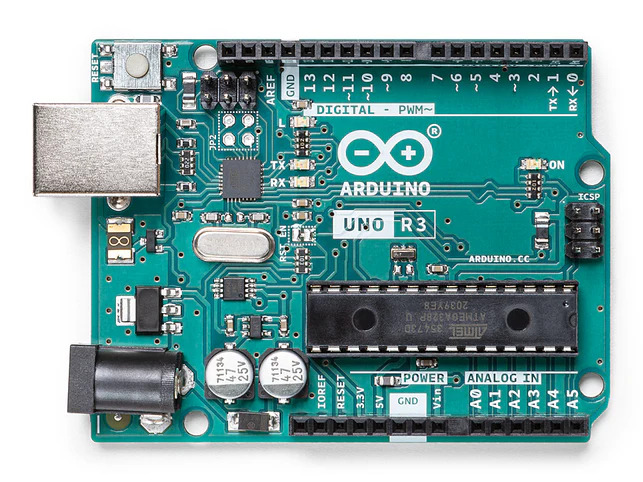
\includegraphics[width=0.45\textwidth]{img/arduino_uno_rev3}
    \hfill
    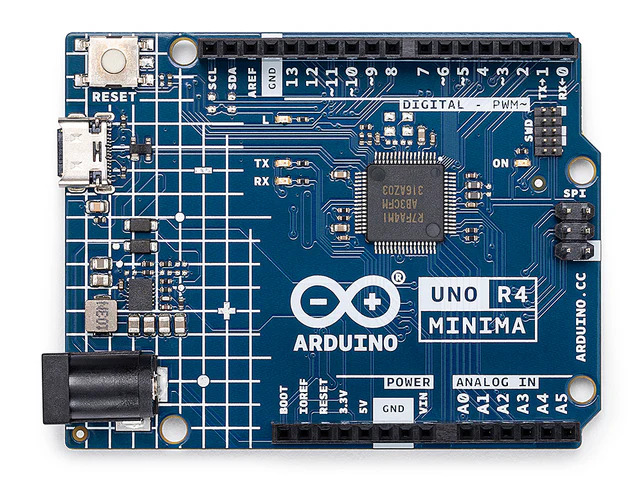
\includegraphics[width=0.45\textwidth]{img/arduino_uno_rev4}
    \hfill
    \\ \scriptsize
    Source: \url{https://store.arduino.cc/collections/edu-boards}, under the \href{https://creativecommons.org/licenses/by-sa/3.0/legalcode}{Creative Commons Attribution ShareAlike 3.0} license.
    \caption{Arduino Uno Board Revisions R3 and R4 Minima.}
    \label{fig:arduino_uno}
  \end{wide}
\end{figure}

\begin{figure}
  \begin{wide}
    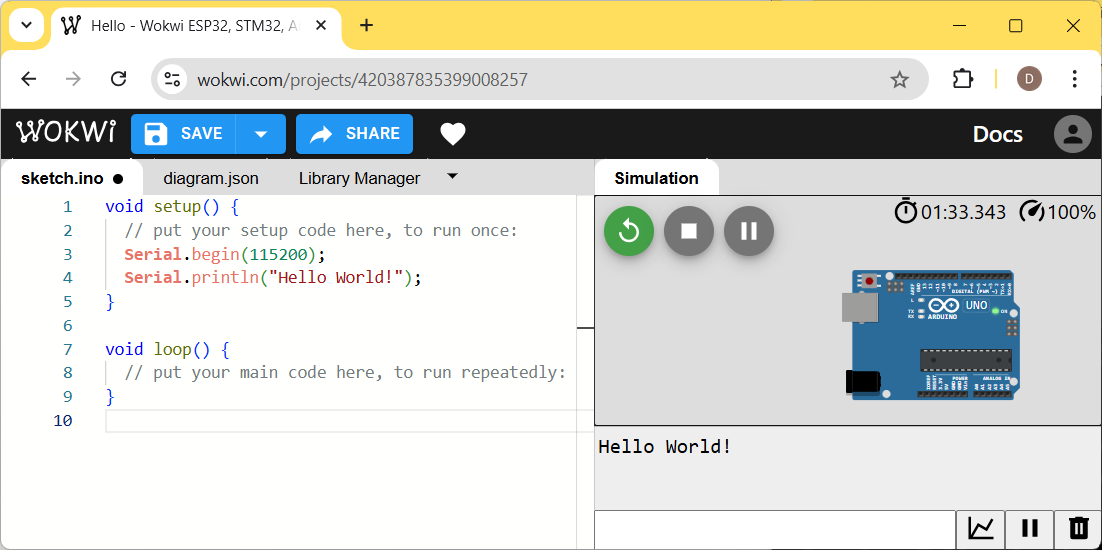
\includegraphics[width=\textwidth]{img/wokwi-hello.png}
    \\ \scriptsize
    Access this on \url{https://wokwi.com/projects/420387835399008257}
    \caption{Hello World program on the Wokwi simulator.}
    \label{fig:wokwi-hello}    
  \end{wide}
\end{figure}

%%% Local Variables:
%%% TeX-master: "main"
%%% eval: (adaptive-wrap-prefix-mode t)
%%% eval: (visual-line-mode t)
%%% eval: (nlinum-mode t)
%%% TeX-engine: luatex
%%% End:
